% PLEASE FOLLOW POSTED GUIDELINES!!

% Please see the two LAr CDR 'guidelines' writeboards in basecamp
% at https://lbne-doc.basecamphq.com/projects/4264323/writeboards
% One is for text, the other for images and figures 

%%%%%%%%%%%%%%%%%%%%%%%%%%%%%%%%%%%%%%%%%%%%%%%%%%%%%%%%%%%%%%%%%%%%%%%%
%%%%%%%%%%%%%%%%%%%%%%%%%%%%%%%%%%%%%%%%%%%%%%%%%%%%%%%%%%%%%%%%%%%%%%%%
\chapter{Data Acquisition}
\label{ch:trig}

The scope of the data acquisition (DAQ) subsystem includes the 
design, procurement, fabrication, testing, delivery and installation 
of a combination of custom and commerical electronics modules, (including 
commodity computing and networking hardware), as well as both commercial 
and internally developed software. 

\begin{editornote}
  Editor's Note: This chapter has not been updated since 2012, with the exception of this note.  Most of the
text from 2012 is no longer valid. \\

The data acquisition system has been evolving since the 2012 design. The design for the 35-ton prototype, the most recent,
 is based on artdaq, a toolkit for building DAQ systems that provides core DAQ functions. Experimenters leverage the infrastructure it provices and are able to focus on developing artdaq-compatible software modules to perform functions specific to the experiment. \\ 

Artdaq has been developed at Fermilab and is in use in several other experiments.  It has been the default choice for the DAQ framework for the full LBNE detector for some time. \\ 

LBNE collaborators have so far developed modules that configure and read out the RCE and SSP boards that are connected to the TPC and photon system detectors, respectively, for the 35-ton detector.  They are also developing reconstruction and filtering software modules that will analyze the data as it is acquired.  \\ 

This artdaq-based DAQ system %for the 35-ton detector 
has been successfully used to acquire data in electronics and detector integration tests for the 35-ton prototype.   As part of this, a preliminary design has been developed for the full detector. The design uses a two-stage artdaq system to stream zero-suppressed data into a farm of processes, run software modules to find events of interest, and use the results of this software trigger to initiate the readout of all of the data produced for the events of interest. \\ 

Since artdaq uses art, the same event analysis framework can be used online and offline.  This allows experimenters to develop and substantially test their software in an offline environment and only include the full DAQ infrastructure for final testing.
\end{editornote}



\section{Introduction}
The DAQ subsystem will perform the primary functions of:

\begin{itemize}
  \item Configuration, online calibration/checkout, and control of 
        operations of detector subsystems, including the generation 
        and distribution of timing and control signals,

  \item Readout of raw data from the TPC and other detector subsystems,  

  \item Filtering the data and constructing event records to be 
        logged to persistent storage media, 

  \item Control of, and readout of data from, devices 
        providing real-time information on detector, subsystem 
        and environmental conditions,  

  \item Providing user/operator interfaces for these functions via 
        a run control system, and

  \item Receiving and handling the LBNE beam-spill signal.
\end{itemize}

In this chapter, a reference design for the DAQ subsystem is presented.  
The development of this design is guided by recent experience gained 
in the development of relevant systems for the NO$\nu$A~\cite{novatdr} 
and MicroBooNE~\cite{microboonecdr} experiments, as well as from 
running experiments with comparable channel counts and/or experimental 
conditions, such as D-Zero, CDF, MINOS and ICARUS.

%\section{Description}

The DAQ subsystem is to be located external to the cryostat vessel, with 
components in the detector hall and in an on-site control room.  The 
primary interface is with the TPC front-end electronics.  Additional 
interfaces are with the front-end electronics systems for the 
%Scintillation 
photon-detector subsystem, with the Fermilab Accelerator complex 
(the beam-spill signal), and with the cryogenics subsystem (for logging of 
conditions).  

%\fixme{A pgraph on what DAQ DOES include, first?} I moved the following up from further down.

The DAQ subsystem reference design described in this chapter 
consists of the following components:
\begin{itemize}
  \item custom `Data Concentrator' modules located in the detector hall to 
        receive data from the TPC (transmitted via redundant LVDS lines) 
        and to carry out low-level data processing operations (these connect 
        to the network, listed next)
  \item a network consisting of commercial ethernet switches located 
        in the detector hall and a commercial router located in the 
        counting house/control room, (for the transmission of data to the farm, listed next)
  \item a local farm of commodity computers that provide trigger 
        event-building and 
        real-time processing/event reconstruction functions
  \item a custom timing system consisting of a master unit that locks onto a 
        GPS clock and distributes timing signals to the data concentrator 
        modules via slave units 
  \item dedicated computer nodes that host run control, routing control, 
        node supervisor and slow controls processes
\end{itemize}
%
The DAQ subsystem does not include power-supply hardware 
for the TPC or front-end electronics, nor does it include the 
cryogenics subsystem process-control and monitoring functions.


\section{Design Considerations}

\subsection{Physics Considerations}

Physics considerations determine the scale of the primary 
tasks of digitized TPC data readout, event building and online processing. 
In addition to rates for processes of interest, the DAQ subsystem design 
depends critically on the specifications for the TPC and front-end 
electronics systems, chosen to satisfy the LBNE physics requirements.  
As described in Chapter~\ref{ch:tpc}, obtaining sensitivity to 
signals that occur independently of the LBNE beam spill, 
such as those from nucleon decay or supernova-neutrino bursts, 
requires a free-running transmission of data from the TPC front-end 
electronics.  The sampling rate of 2~MHz has been chosen so as to 
achieve the required position resolution along the ionization drift 
direction.  
The task of data transfer is facilitated by multiplexing and 
data compression/zero-suppresion in front-end ASICs in the LAr, 
and by redundant data lines that provide connection to data-acquisition 
hardware located outside the cryostat.  With these specifications, 
event building and triggering/filtering can be accomplished outside the 
cryostat.  The LBNE beam-spill signal and data from the photon-detection 
system are considered part of the 
data stream, and can be used at this stage to select events for processing 
and storage through physics-specific data streams, as desired.

\subsection{Technical Considerations}
In addition to physics considerations, DAQ design goals include  
minimizing the impact of single-point failures and maximizing 
the use of commercial components.  
For the reference design described here, sited at the 4850L of the Sanford Laboratory, the 
atmospheric-muon rate is small enough -- 0.1~Hz within the full LAr-FD active 
volume -- to contribute only negligibly to the DAQ bandwidth requirement.
For reference, the rate at the alternate 800L site 
is estimated to be 500~Hz within the active volume.  
This and other assumptions are discussed below in 
Section~\ref{sec:v5-daq-assumptions}.  The requirements on the DAQ system are listed in the
requirements documentation~\cite{lar-fd-req}.





\subsection{Event Rates and Timing}
\label{sec:v5-daq-assumptions}

%The DAQ subsystem design depends on assumptions pertaining to physics goals as well as detector configuration and conditions. 

Signals associated with beam events will be localized within the 
TPC and synchronous with discrete (${\cal O}(1\,s)$ rep rate) 
beam-spill intervals spanning 
approximately $10\,\mu s$.  
However other physics events of interest will occur at random 
times, and can be dispersed throughout the TPC volume as in the case 
of neutrino bursts from supernovae.  Other specific signatures, such 
as very slow-moving magnetic monopoles ($\beta < 10^{-3}$) may involve 
signals spanning sample times exceeding the 2.3-ms maximum ionization-drift time.  

Cosmic-ray muons dominate the physics rate, even at the proposed 4850L site.  
However, this rate is negligible with respect to noise sources.  This is not 
the case at other possible detector depths:  
at the alternate site identified at 800L, the total 
rate in the detector is estimated to be approximately 500~Hz, accounting 
for variations in overburden due to topography at the prospective cavern 
site, while 
the rate at the 300L is expected to be higher than this by a factor of 10.  
%These estimates are in the process of being improved with more detailed 
%calculations/simulations.  
For shallow depths, the frequency of muon incidence is 
comparable to the maximum duration (2.3~ms) of the signal from an event, 
and hence cosmic-ray muons would have an impact on 
the required bandwidth of the DAQ system:  while the system described 
here has sufficient bandwidth to operate at depths as shallow as the 
identified 800L site, going shallower still would impact the design.

As described earlier in this report
%\fixme{reference actual section.  
%JU response: doesn't the figure reference provides this?} 
(see Figure~\ref{fig:tpc-elec-schematic}), 
the cold electronics for a single Anode Plane Assembly 
will consist of twenty 128-channel Front-End Readout 
Boards, each providing a single digital input to a 20-channel
Data Output Board, which includes a 20$\times$ MUX stage into a  
driver for a redundant pair of LVDS outputs.   

The Front-End Boards will generate zero-suppressed data: worst-case 
scenarios (i.e., $>10\,$GeV EM showers contained within a single APA) 
indicate roughly a factor of ten reduction in the number of samples 
read out with respect to the maximum (2304 wires $\times$ 4625 0.5-$\mu$s 
samples per wire).  
%For cosmic-ray muons, at $\sim 3.4\,$Hz per APA the 
%highest-rate physics process, the rejection factor is estimated to be 
%$\sim 200$.  
For cosmic-ray muons, the rejection factor is estimated to be $\sim 200$.  
The rejection factor is of course much higher in APAs 
not containing any portion of a physics event.  Radioactive decay 
from $^{39}$Ar and $^{85}$Kr in the LAr, and to a lesser extent from 
detector materials (U/Th/Co/K), is estimated to provide a
65-kHz/APA rate of activity of energy above about 300~keV (0.3 MIPs) 
but less than $\sim 5\,$MeV, while 
electronics noise (assuming 10:1 S/N for 1 MIP, and a threshold of 0.3 MIPs) 
will contribute a relatively low rate per APA of singles.  
Table~\ref{tbl:daq-signal-rates} provides a summary of these rate 
estimates.  Work is ongoing to further refine them.
%
\begin{table}[htbp]
  \begin{center}
  \caption[Rates and data sizes/rates for various processes.]
          {Per-APA estimates of rates and data sizes/rates for various 
           processes.  
           Unless otherwise stated, estimated numbers of samples and 
           data rates assume suppression of signals below 0.3 MIP.  
           `Inst.\ Data Rate' refers to the number of bits in a 2.3-ms 
           long data block divided by this time interval, while `Avg.\ 
           Data Rate' factors in the process rate.  
           A 12-bit ADC is assumed, and no allowance is made for data items such as 
           time-stamp, channel identifier, etc.}
  \label{tbl:daq-signal-rates}
  \begin{tabular}{|l|c|c|c|c|} \hline
    {\bf Process} & {\bf Rate } & {\bf Samples}
                  & {\bf Inst.\ Data } & {\bf Avg.\ Data}  
                  \cr 
                  & {\bf (kHz/APA)}  & {\bf (per APA)}
                  & {\bf Rate (Mbps)} & {\bf Rate (Mbps)} \cr \hline
    Generic 2.3 ms interval 
                  & 0.43 & $1.06 \times 10^7$ 
                  & 55,000 & 55,000 
                  \cr 
                  (not zero-suppressed) & & & & \cr \hline
    Cosmic ray muons (4850L)
                  &  $6\times 10^{-7}$ & $5 \times 10^4$ 
                  &  260 & $1\times 10^{-4}$
                  \cr 
                  & & & & \cr \hline
    Cosmic ray muons (800L)
                  &  0.0034 & $5 \times 10^4$ 
                  &  260 & 2.0 
                  \cr 
                  & & & & \cr \hline
    10 GeV EM shower 
                  &  --- & $1 \times 10^6$
                  & 5,200  & --- 
                  \cr
                  & & & & \cr \hline
    Radioactivity: U/Th ($\gamma$'s)
                  & $\sim 1$ & 40
                  & 0.48  & 0.48
                  \cr
    \phantom{Radioactivity: }$^{39}$Ar/$^{85}$Kr ($\beta$'s)
                  & 63 & 24
                  & 18  & 18
                  \cr
                  & & & &  \cr \hline
    Electronics noise
                  & $\sim 1$ & 15 
                  & 0.2  & 0.2 
                  \cr 
                  (not common mode) & & & & \cr \hline
  \end{tabular}
  \end{center}
\end{table}


It can be concluded from the table that the average data rates out of the 
front-end electronics system are manageable: 
about 20 Mbps of `salt and pepper' per APA 
due to radionuclides in the Ar and TPC materials. 
Large beam- or atmospheric-neutrino interactions or 
showering ultra-high-energy cosmic-ray muons will result in high (Gbps-level)
instantaneous rates on the scale of the maximum ionization drift period, 
but contribute negligibly to the average rate.
With sufficient buffering in front-end ASICs, as described 
in Chapter~\ref{ch:tpc}, the plan of having a single LVDS output line per APA 
(plus a second one for redundancy) is easily realizable.  However, 
to be conservative, and to provide opportunities for collecting data with 
relaxed zero-suppression, the DAQ reference design described below 
allows for as many as 20 output lines per APA (one per front-end board), 
each operating below 24~Mbps.  This leads to a capacity for APA output 
rates up to 480~Mbps, well above the $\sim 20$ Mbps expected. 




%%%%%%%%%%%%%%%%%%%%%%%%%%%%%%%%%%%%%%%%%%%%%%%%%%%%%%%%%%%%%%%%%%%%%%%%
%%%%%%%%%%%%%%%%%%%%%%%%%%%%%%%%%%%%%%%%%%%%%%%%%%%%%%%%%%%%%%%%%%%%%%%%
\section{Architecture Summary}
\label{sec:v5-trig-daq}

The reference design of the DAQ system is summarized in 
block diagram form in Figure~\ref{fig:daq-block-diagram}.  
Component counts are given in Table~\ref{tbl:daq-component-counts}.  The main 
elements of the design are described in the following sections.
%
\begin{figure}[htbp]
\centering
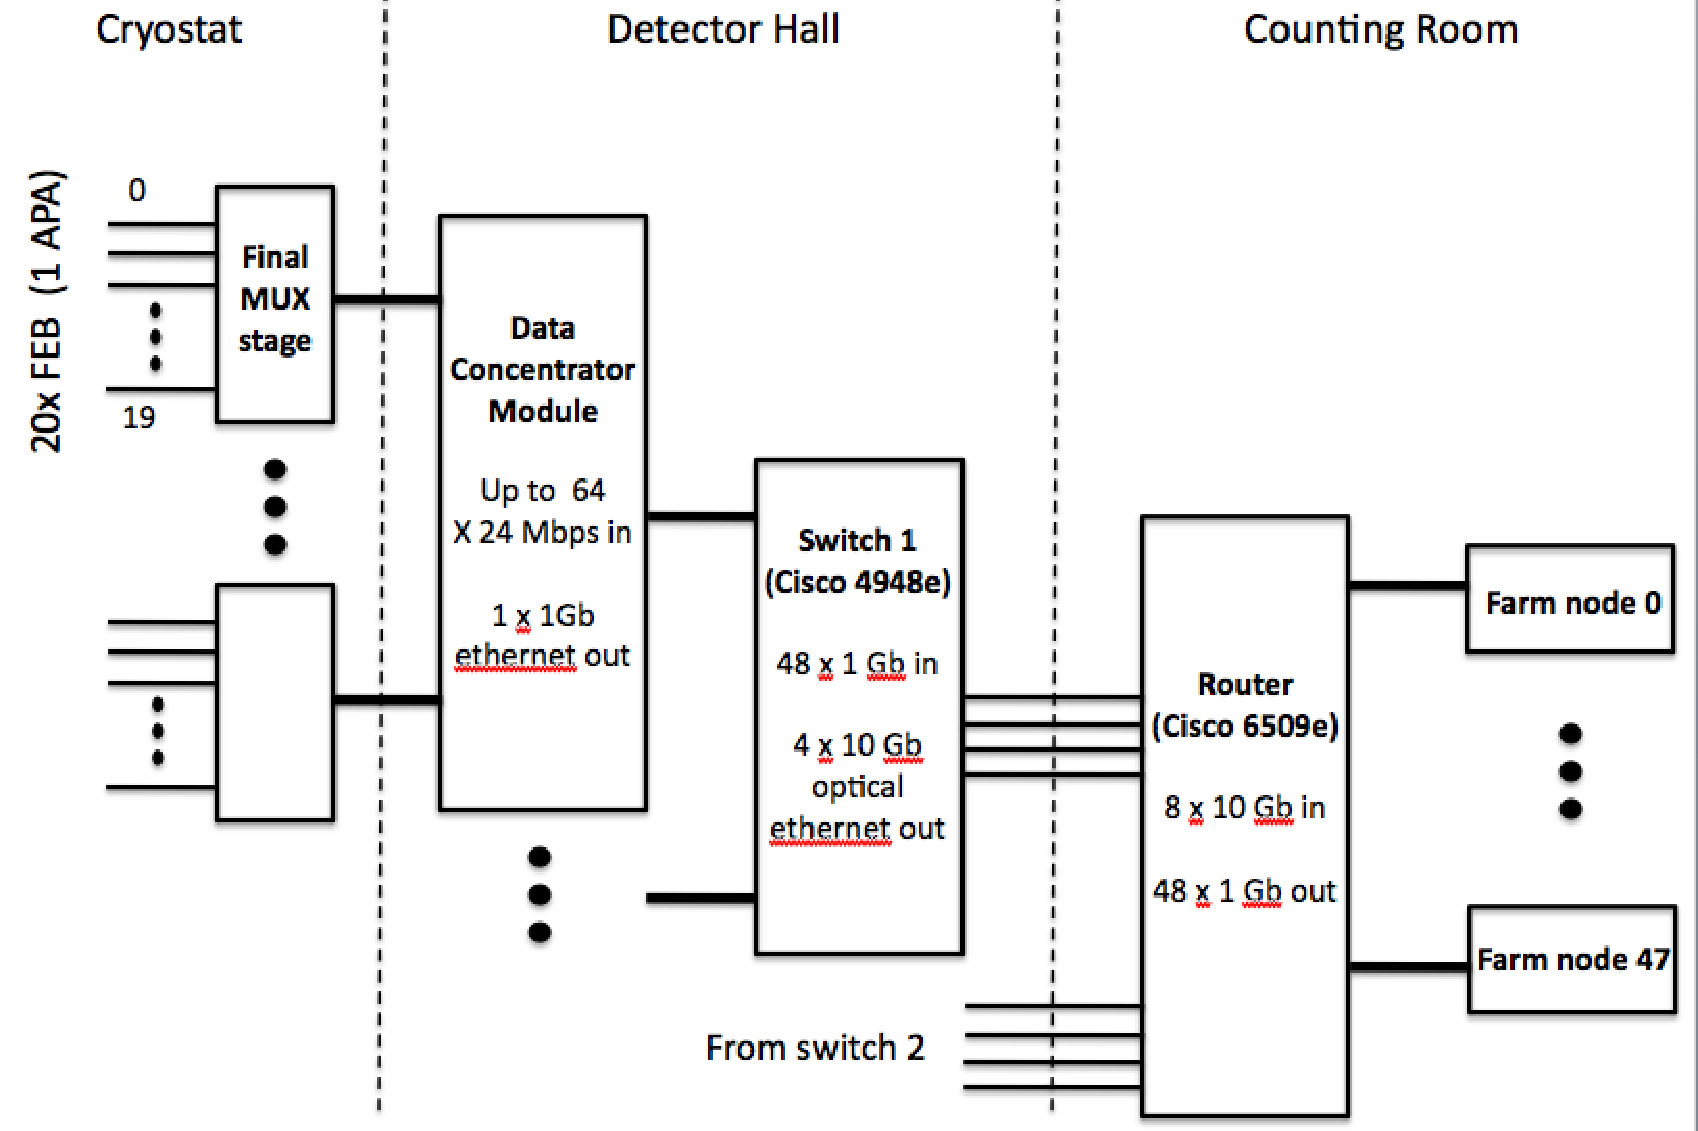
\includegraphics[width=\linewidth]{v5c4-daq-block-diagram}
\caption{Block diagram depicting the DAQ reference-design architecture}
\label{fig:daq-block-diagram}
\end{figure}
%
\begin{table}[htbp]
  \begin{center}
  \caption[DAQ subsystem component counts]
          {DAQ subsystem component counts for one 20-kton 
           module/cryostat.  The total component count for the 
           two-cryostat LAr-FD will be twice 
           what is shown.}
  \label{tbl:daq-component-counts}
  \begin{tabular}{|l|r|} \hline
    {\bf Quantity} & {\bf Description} \cr \hline
    54  & Data Concentrator Modules \cr \hline
    2   & Ethernet Switches (Cisco 4948E or similar) \cr \hline
    1   & Ethernet Switch Chassis (Cisco 6509E or similar), with \cr 
    1   & 8-port input optical 10-GB ethernet interface module, and \cr
    1   & 48-port output 1-GB ethernet interface module \cr \hline
    48  & Data Farm compute nodes \cr \hline
    1   & Readout Supervisor compute node (not shown in Figure)\cr \hline
    1   & Routing Master compute node (not shown in Figure)\cr \hline
    1   & Master timing unit + GPS receiver (not shown in Figure)\cr\hline
    9   & Slave timing units (not shown in Figure)\cr\hline
    1   & Run Control compute node (not shown in Figure)\cr \hline
    1   & Slow Controls compute node (not shown in Figure)\cr \hline
  \end{tabular}
  \end{center}
\end{table}


%%%%%%%%%%%%%%%%%%%%%%%%%%%%%%%%%%%%%%%%%%%%%%%%%%%%%%%%%%%%%%%%%%%%%%%%
%%%%%%%%%%%%%%%%%%%%%%%%%%%%%%%%%%%%%%%%%%%%%%%%%%%%%%%%%%%%%%%%%%%%%%%%
\section{Data Concentrator Module}
\label{sec:v5-trig-datatransfer}

The LBNE/LArTPC Data Concentrator Module (DCM) serves as the primary interface 
between the cold TPC electronics and the DAQ subsystem, with the main task 
of receiving serial data pushed out of the front end.  It also packetizes and 
transmits the data to `data farm' computers for event 
building via an ethernet switch array, described in 
Section~\ref{sec:v5-trig-switch}.  Finally, it will provide the interface 
for transmitting timing and control signals to the cold electronics. 
As such, it is envisioned to provide the functionality of NO$\nu$A's custom 
electronics module of the same name, and similarly, the digital portion 
of MicroBooNE's ``Front End Module'' (FEM) cards.  

For the purposes of this conceptual design, the NO$\nu$A DCM 
is considered as is.  Several NO$\nu$A prototype modules are shown in 
Figure~\ref{fig:daq-dcm-photo}.  The NO$\nu$A DCM consists of 64 input 
ports (RJ45 sockets), and a single 1~GB output line.  A large 
FPGA provides preliminary data processing capability.  A processor (running 
Linux) provides local control for configuration, buffering and routing 
functions.
%
\begin{figure}[htbp]
\centering
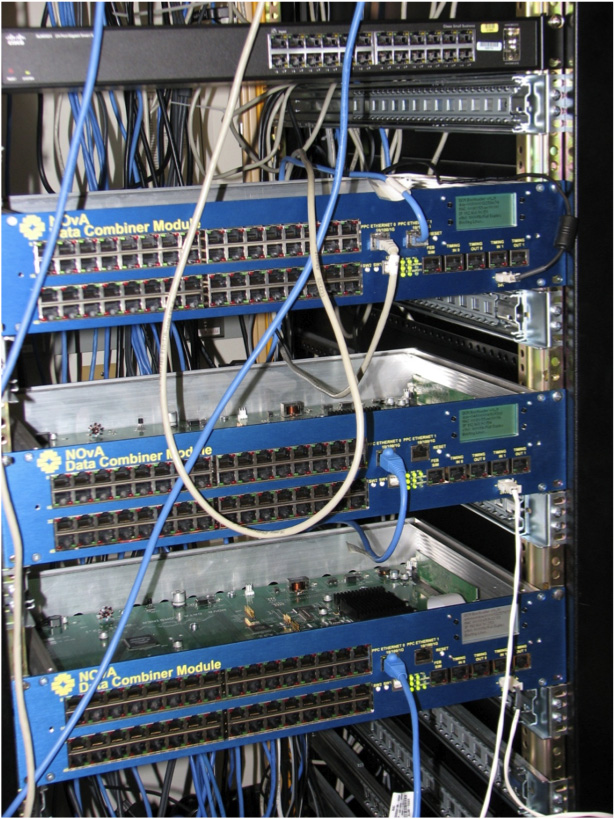
\includegraphics[width=0.4\linewidth]{v5c4-daq-dcm-photo}
\caption{Photograph of several prototype NO$\nu$A Data Concentrator Modules.}
\label{fig:daq-dcm-photo}
\end{figure}


Assuming the Data Output Board is implemented in the cold volume with 
20$\times$ muxing to provide a single output line per APA, only a handful 
of NO$\nu$A-style DCMs would be required to read out the entire detector.  
Considering typical data rates of order 20~Mbps per APA 
(see Table~\ref{tbl:daq-signal-rates}), the 1~Gb (80 MB/s) 
DCM output bandwidth 
could comfortably accommodate more than a few APA's.
More likely, the LBNE DCMs would be designed for fewer input lines 
in this case, in order to distribute them rationally. 

On the other hand, allowing for the possibility of 20 output lines per APA, 
the NO$\nu$A DCM footprint is well matched to the LBNE APA granularity.  In 
this case, a single DCM could serve two or three APAs.  Outputs from auxiliary 
detector elements could make use of the otherwise unused DCM input channels.
To obtain a conservative estimate of costs, this configuration is considered 
with two APA's per DCM.


\subsection{Data Processing/Handling}
%: demuxing, unpacking, additional zero suppresion} -- too long a title

As currently imagined, buffers in the front-end electronics will constitute  
a source of variable-length (i.e., zero-suppressed) time-ordered sequence 
of samples for each channel (wire) registering activity, along with a 
channel address and time stamp.  Although this format is likely to be 
suitable for transmission to the data farm, the DCM's task of generating 
ethernet packets also provides an opportunity for additional data processing.  
If re-formatting or additional zero suppression is desired, 
it could be done here.   


%As described in Chapter~\ref{ch:tpc}, zero-suppressed digitized signals from 
%a single APA will arrive on an LVDS lines and, for redundancy, 
%on four 'primary' optical lines and four 'backup' optical lines.  
%Thus, for example, each LVDS line will carry a serial stream of data 
%with a common timestamp from 128 wires once every $0.5\,\mu s$, for a 
%net rate of 384 Mbps. 
%As is the case for MicroBooNE, analysis of the complex time structure 
%of the ionization signature for a given induction or collection wire 
%requires that data be `rotated' into a time-ordered data set, spanning 
%a specified time frame.  In the case of MicroBooNE the nominal time frame 
%is a $4\, ms$ interval; it remains to be determined what interval is 
%appropriate for LBNE.  The deserialization and rotation of the data 
%can be accomplished in an FPGA as is the case in the MicroBooNE FEM.
%It also remains to be determined whether (further) zero suppression 
%can/is desired take place at this stage.  

%\subsection{Output data}
%
%As described below in Section~\ref{sec:v5-trig-evtbuild}, the output of 
%the Data Receiver system will be transfered to a disk farm 
%(``Buffer Farm'') for event building and triggering.  NOvA achieves this 
%with Gigabit Ethernet links, and a processor on the Data Concentrator 
%that forms the packets.  The viability of a similar scheme for LAr20 
%will depend on the degree of data reduction upstream of this step.  
%({\bf Need some better numbers here!})  In a worst-case scenario 
%- no zero-suppression and only the 8:1 lossless compression in the front-end 
%ASIC - the LVDS output (30 channels) from a single APA would correspond to 
%11.5 Gbps to be moved out to the Buffer Farm.  Only a small number 
%of detector channels will have a real signal in a physics event of interest, 
%and then only for a small fraction of the samples collected during a 
%given time frame.  Thus even a very conservative zero suppression scheme 
%realized in the front-ends and/or in the Data Receiver could reduce this 
%to a manageable level.  A challenge will be how to fold in data from 
%`large' events (e.g., from calibration/random noise sources) without 
%introducing deadtime for the DAQ system.

\subsection{Timing, Control and Configuration Signals}

The DCM will provide the interface for the transmission of 
timing, control and configuration signals to the TPC/front-end electronics.
More detail on these signals is given in following sections.

%%%%%%%%%%%%%%%%%%%%%%%%%%%%%%%%%%%%%%%%%%%%%%%%%%%%%%%%%%%%%%%%%%%%%%%%
%%%%%%%%%%%%%%%%%%%%%%%%%%%%%%%%%%%%%%%%%%%%%%%%%%%%%%%%%%%%%%%%%%%%%%%%
\section{Ethernet Switch Network}
\label{sec:v5-trig-switch}

The network accomplishing transmission of data from DCMs to the data 
farm will consist of two layers of ethernet switch arrays.  
The first level will reside in the detector hall, and is imagined to be 
able to operate with little external control.  Commercial switch modules 
such as the Cisco 4948E are well suited for this application.  The 4948E 
has 48 1-GB input ports and four 10-GB optical output ports, 
as well as 175~MB of buffer memory.  Two modules will support the 
required data throughput for the entire detector.

The second level will be deployed in the counting room and will 
serve as a router to the data farm nodes located there.  For this application 
the Cisco 6509E switch chassis provides a possible implementation.  This 
would be loaded with a single 8-port 10 GB blade for input data from the 
4948E's, and a single 48-port 10/100/1000~MB blade for 1-GB output to 
farm nodes.

Routing information will be provided to DCMs by a Routing Master.  This 
task will run on a computer located in the counting room.  It will monitor 
the state of data farm nodes, and provide routing information to DCMs.


%%%%%%%%%%%%%%%%%%%%%%%%%%%%%%%%%%%%%%%%%%%%%%%%%%%%%%%%%%%%%%%%%%%%%%%%
%%%%%%%%%%%%%%%%%%%%%%%%%%%%%%%%%%%%%%%%%%%%%%%%%%%%%%%%%%%%%%%%%%%%%%%%
\section{Event Building and Triggering}
\label{sec:v5-trig-evtbuild}

The event building and triggering function of the LAr-FD DAQ system 
will be performed by the data-farm computers.  Event data will be staged 
locally before being transmitted in quasi real-time (nominally to Fermilab) 
for archival to persistent storage. 

\subsection{Event Building}

At present it is imagined that an event will consist of raw data from the 
entire detector, spanning a time interval yet to be determined.  To construct 
such an event, DCM packets corresponding to data with a common (range of) 
timestamp value(s) will be routed to a particular data-farm node.  

An alternate scenario considers events as being localized to individual 
APAs, or possibly small APA clusters.  Individual farm nodes would work 
only on the corresponding data to generate event records.
This concept is attractive in that (1) the routing of data to farm nodes 
is simplified, and (2) event record sizes are kept as small as possible.  
The main drawbacks are that (1) offline processing/analysis of these event 
records for physics events with activity spanning geographical 
boundaries would become more cumbersome; (2) certain physics studies, such 
as proton-decay searches, might benefit from 
%find it useful if 
simple access to data-registering activity in remote sections of the detector 
%were provided
; and (3) auxiliary data  
would either be unnecessarily duplicated or 
would have to be stored in its own event record, again adding complexity 
to the data-analysis process.  Evaluation of this alternative is ongoing.

\subsection{Event Data Model}

We will need to develop an Event Data Model (EDM).  It may be advantageous 
to implement the raw data EDM in a custom format, as opposed to one based on 
ROOT.  Experience with MicroBooNE will be helpful in optimizing the design 
for this.

\subsection{Triggering and Selection for Output Streams}

Significant work remains to understand how data-farm nodes will carry out 
event filtering and creation of separated physics/task-specific data 
streams.  
%prev phrase a bit confusing AH
Use of the LBNE beam-spill signal to identify events recording 
beam-induced activity is expected to be straightforward.  However, 
identifying events of interest that lack such a signal requires study.  
Is it sufficient to find a suitable way to generically veto events based 
on lack of coherent detector activity, or must `positive' signatures for 
each of the physics processes of interest be identified for triggering?  
To indicate the range of signatures, 
these processes of interest include, for example, (1) beam-induced events 
for which the corresponding beam-spill signal is missing due to 
network failure or other malfunction, (2) atmospheric-neutrino interactions, 
(3) supernova-neutrino bursts, (4) proton decay, and (5) magnetic-monopole 
incidence.  
%Additionally, what are the requirements for storage of cosmic-ray 
%muon events, either for detector calibration or physics studies?

\subsubsection{Rejection of Event Records}

%For the reference DAQ system design described here, it is assumed that 
%cosmic-ray muons will not be prescaled in the primary output-data stream.  
%This assumption is key in two ways.  First, for a cosmic-ray muon rate of 
%200~Hz over a full 20-kt detector module, 
%a significant fraction of  $2.3\,ms$-long intervals 
%will contain activity from a cosmic-ray muon in some portion of 
%the detector.  Second, not having to identify and reject cosmic-ray muons 
%suggests that simple trigger primitives can be 
%generated and combined in such a way as to reject most of the 
%remaining 
%($85\%$ for the case of record time frames of $2.3\,ms$)  
%`record time frames' hard to parse AH -- is it time frames that are recorded?
Since the dominant rate is due to dispersed low-energy activity 
associated with radionuclide decays, simple trigger primitives can be 
generated and combined so as to reject event records failing well-defined 
(and easy-to-model) criteria.  
For example, event records in which no APAs 
register energy deposition in excess of some threshold (say 5~MeV) 
will be sufficient to reject most background events.

\subsubsection{Event selection for Physics-Specific Streams}

Even given the above statements about event rejection, it is desired to 
perform some type of high-level event reconstruction to identify candidates 
compatible with specific physics signatures.  This level of analyses is 
essential both for online detector performance diagnostics as well as 
for the case where candidate event records of particular types are to be 
written to parallel output streams.  For the former application, 
an unanticipated shortfall in the DAQ data farm computing capacity 
could be easily addressed through establishment of a separate computer farm 
for online analysis.
For the latter application, it would be necessary to adjust the size of 
the data farm depending on the processing requirements.  These are not 
known at this time.  However, with anticipated costs for commodity 
computing systems, it is not expected that the overall cost of the 
DAQ/online computing systems would increase significantly relative to 
the currently budgeted system.%AH only read in cursory manner 10/20

%%%%%%%%%%%%%%%%%%%%%%%%%%%%%%%%%%%%%%%%%%%%%%%%%%%%%%%%%%%%%%%%%%%%%%%%
%%%%%%%%%%%%%%%%%%%%%%%%%%%%%%%%%%%%%%%%%%%%%%%%%%%%%%%%%%%%%%%%%%%%%%%%
\section{Timing System }
\label{sec:v5-trig-timing}

Comparable requirements and conditions suggest a timing system 
similar to that being implemented for NO$\nu$A.  That system meets the 
requirements of deterministic timing and coherence of signals distributed 
across the entire detector.   It consists of a Master Timing Unit (MTU)
whose main task is generation of GPS-based timing packets, and an 
array of Timing Distribution Units (TDUs).  The TDUs are geographically 
distributed: they compensate for propagation delays before transmitting 
timestamp packets to the front ends via DCMs.  Such a system could work 
well for LBNE and may be able to be adapted with only minor 
design modifications.  For NO$\nu$A, each TDU is associated with 12 DCMs; 
for LBNE a reasonable distribution could be achieved with 9 TDUs, 
one for every 6 DCMs (i.e., spaced at intervals of 5~m along the 
length of the detector).

%%%%%%%%%%%%%%%%%%%%%%%%%%%%%%%%%%%%%%%%%%%%%%%%%%%%%%%%%%%%%%%%%%%%%%%%
\section{Run Control }
\label{sec:v5-trig-runcontrol}

The scope of 
functionality of the Run Control system includes operation of DAQ 
subsystem components, configuration 
of front-end electronics, control of power supplies and other auxiliary 
equipment, and control of data collection.  Development of a 
user interface for experimenters during data-taking and for technical 
personnel to assist with commissioning and debugging activities is key.  To date, 
limited effort has been put forth in the design of the Run Control system.
To the extent that the challenges faced are similar to those that have 
been addressed at MINOS and ICARUS, no technical obstacles are foreseen.  
As the designs of the DAQ and other subsystems continue to develop, 
specifications of the Run Control system will become more concrete.

%%%%%%%%%%%%%%%%%%%%%%%%%%%%%%%%%%%%%%%%%%%%%%%%%%%%%%%%%%%%%%%%%%%%%%%%
%%%%%%%%%%%%%%%%%%%%%%%%%%%%%%%%%%%%%%%%%%%%%%%%%%%%%%%%%%%%%%%%%%%%%%%%
\section{Slow Control Systems }
\label{sec:v5-trig-slowcontrol}

The Slow Control system is a critical element of the DAQ, providing the 
main interface to power supplies for the detector and electronics as well  
as to equipment used to monitor the operational status of the detector and 
supporting systems.  As in the case of the Run Control system, the 
development of the conceptual design for the Slow Control system is in 
its early stages.  Again, based on experience from other experiments, 
no obstacles are foreseen with regard to the development of a robust 
system.

%%%%%%%%%%%%%%%%%%%%%%%%%%%%%%%%%%%%%%%%%%%%%%%%%%%%%%%%%%%%%%%%%%%%%%%%
%%%%%%%%%%%%%%%%%%%%%%%%%%%%%%%%%%%%%%%%%%%%%%%%%%%%%%%%%%%%%%%%%%%%%%%%
\section{DAQ Infrastructure }
\label{sec:v5-trig-infrastructure}


\subsection{Wide Area Network}

As in the case of MINOS and NO$\nu$A, it is expected that event data can be 
transmitted over the network to Fermilab.  Although rates for events of 
interest are comparable, data throughput for the LBNE LArTPC is 
expected to be at least an order of magnitude higher.  A detailed 
analysis of the requirements of Sanford Laboratory for the appropriate level of 
connectivity within and off the lab site will need to be carried out.

\subsection{Online Data Storage}

To protect against signficant periods of absent network connectivity, it 
is desired to store a significant amount of the data emerging from the 
DAQ to local storage.  A local data storage facility of $\sim 100\,$TB is 
expected to be more than adequate for five days worth of detector data, 
even without prescaling cosmic-ray muon events.

\subsection{Power and Cooling}

Power and cooling requirements for the DAQ system described here are 
modest.  DCMs operate at below 50~Watts each, while the maximum power 
consumed by each of the two Cisco 4948Es is 275~Watts.  Assuming 
power supplies that operate at 75\% efficiency, and accounting for 
other components, the total DAQ subsystem budget for power 
in each 20-kton detector/cryostat hall is likely to be below 15~kW.

%%%%%%%%%%%%%%%%%%%%%%%%%%%%%%%%%%%%%%%%%%%%%%%%%%%%%%%%%%%%%%%%%%%%%%%%
%%%%%%%%%%%%%%%%%%%%%%%%%%%%%%%%%%%%%%%%%%%%%%%%%%%%%%%%%%%%%%%%%%%%%%%%

